\documentclass{article}
\usepackage{ctex}
\usepackage{tikz}
\begin{document}
\title{$\sqrt2$是一个无理数}
\maketitle
古希腊数学家曾认为一切数皆整数之比,直到他们发现$\sqrt2$这个反例。这个事实用今天的话说$\sqrt2$是一个十数无理数,用欧几里得的话说 1 和$\sqrt2$是不可公约的。实际上欧几里得会说正方形的边长和对角线是不可公约的。\par

\begin{tikzpicture}[scale=.8,background rectangle/.style=
{draw=blue!50,fill=blue!20,rounded corners=1ex},show background rectangle]
\node[above right]at(0,2.5){\large\textbf{为什么说正方形的边长是$\sqrt2$?}};
\draw(3,0)rectangle+(2,2) (3,0)--+(2,2);
\node[below] at(3,0){1};
\node[right] at(5,1){1};
\node[below]at(4,1){$\sqrt2$};
\node[below right]at(0,2){\parbox{2cm}{(1)由勾股定理,单位正方形的对角线的平方为 2}};

\draw (11,1)rectangle+(2,2) (11,1)--+(2,2)--+(4,0)--+(2,-2)--cycle;
\draw[dotted](13,-1)--+(0,2)--+(2,2);
\node[above]at(12,2){$\sqrt2$};
\node[right]at(13,2){1};
\node[below right]at(6,2){\parbox{3cm}{(2)根据图中面积关系,亦知单位正方形的面积是以对角线为边长的面积的 $1/4$}};
\end{tikzpicture}

可公约以及不可公约都是针对两条线段来说的。设$a,b$是两条线段,$a$不长于$b$,我们用$a$来量$b$,一段一段地量,如果剩下一小段的话,再用这一小段量$a$,这个过程可以一直进行下去,如果有那么一刻,刚好量完不剩下,就说$a,b$是可公约的,否则就说$a,b$是不可公约的。
\par为什么$1$和$\sqrt2$不可公约呢?
\par
\begin{minipage}{\textwidth}\begin{minipage}{0.6\textwidth}
如右图,取$BE=BC$,作$EF\perp BD$交$CD$于$F$,则$DE=EF=FC$(可能不是很显然)。$BC$量$BD$之剩余为$ED$,以$ED$量$BC$同样是以正方形的边长量对角线,无穷无尽。所以正方形的边长与对角线不可公约。
\end{minipage}\quad\begin{minipage}{0.4\textwidth}
\begin{tikzpicture}[scale=.8]
\coordinate[label=above left:$A$](A)at(0,2);
\coordinate[label=below left:$B$](B)at(0,0);
\coordinate[label=below right:$C$](C)at(2,0);
\coordinate[label=above right:$D$](D)at(2,2);
\coordinate[label=above left:$E$](E)at($(B)!1!45:(C)$);
\coordinate[label=below right:$F$](F)at($(E)!1!-90:(D)$);
\coordinate[label=below right:$G$](G)at($(D)!1!90:(E)$);
\draw (B)rectangle(D) (B)--(D) (E)--(F)--(G)--(D);
\end{tikzpicture}\end{minipage}\end{minipage}

\newcommand\proof[1]{\par\vspace*{1em}{\large\bf#1}\par}
\proof{证明$\mathbf{\sqrt2}$是无理数之整除}
反设$\sqrt2=q/p$(既约),则$q^2=2p^2$, $\Rightarrow 2|q \Rightarrow 4|2p^2 \Rightarrow 2|p$,与$q/p$既约矛盾。

\proof{3 进制表示}
设$x=q^2=2p^2$,以 3 进制表示$x$,由于平方数只以 0 或 1 结尾,而平方数的 2 倍只以 0 或 2 结尾,所以$x$以 0 结尾。

\proof{算术基本定理}
把$x$质因数分解,$x=q^2$表明有偶数个 2,$x=2p^2$表明有奇数个 2,矛盾。

\proof{平方为整数}
$2=q^2/p^2$为一整数,所以$p^2|q^2$与$p,q$既约矛盾。

\proof{取出小数部分}
$\sqrt2=q/p$ $\Rightarrow 2q/p=p/q$ $\Rightarrow \{2q/p\}=\{p/q\}$ $\Rightarrow a/p=b/q$ $\Rightarrow \sqrt2=b/a$无穷递归,引发矛盾。

\proof{又一个无穷递归}
$q^2=2p^2 \Rightarrow (2p-q)^2=2(q-p)^2$.

\proof{图形上的无穷递归}
\begin{minipage}{\textwidth}\begin{minipage}{0.6\textwidth}
把边长为$p$的正方形按如图所示的方式放在边长为$q$的正方形内,重合部分的面积等于空白部分的面积,若$q^2=2p^2$,必有$b^2=2a^2$,无穷递归。
\end{minipage}\quad\begin{minipage}{0.4\textwidth}
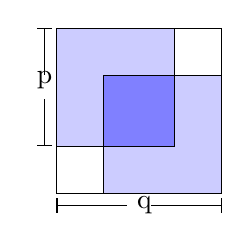
\begin{tikzpicture}[scale=.3]
\draw (0,0)rectangle(7,7);
\filldraw[fill=blue!20](0,2)rectangle(5,7);
\filldraw[fill=blue!20](2,0)rectangle(7,5);
\filldraw[fill=blue!50](2,2)rectangle(5,5);
\draw[|-](-.5,2)--(-.5,4)node[above=0pt]{p};
\draw[|-] (-.5,7)--(-.5,5);
\draw[|-](0,-.5)--(3,-.5)node[right=0pt]{q};
\draw[|-] (7,-.5)--(4,-.5);
\end{tikzpicture}\end{minipage}\end{minipage}

\proof{运用极限}
\def\Crm{\mathrm{C}}\def\Zbf{\mathbf{Z}}
$\sqrt2=q/p \Rightarrow (\sqrt2)^np$总是整数,但$0<(\sqrt2-1)^np=\displaystyle\sum_{k=0}^n\big[\Crm_n^k(\sqrt2)^k(-1)^{n-k}p\big]\in\Zbf$,与$\displaystyle\lim_{n\to\infty}(\sqrt2-1)^np=0$矛盾。

\proof{连分数}
由于$1/(\sqrt2-1)=\sqrt2+1$,知化为连分数是无限长的,所以$\sqrt2$是无理数。

\proof{整系数多项式}
$\sqrt2$为方程$x^2-2=0$的根,由整系数多项式有理根的性质,$\sqrt2$为一无理数。

\proof{艾森斯坦判别法}
$x^2-2=0$在有理数域上不可约,所以$\sqrt2$是无理数。
\end{document}
